\documentclass[11pt]{article}

\renewcommand{\familydefault}{\sfdefault}
\usepackage{sfmath}
\newcommand{\tb}{\textbf}

\usepackage{fullpage}
\usepackage{hyperref}
\usepackage{amssymb}
\usepackage{spalign}
\usepackage{amsmath}
\usepackage{framed}

\newcommand{\R}{\mathbb{R}}

\usepackage[parfill]{parskip}

\hbadness=99999

\hypersetup{
    colorlinks,
    citecolor=black,
    filecolor=black,
    linkcolor=black,
    urlcolor=black
}
\urlstyle{urlcolor=blue}
\usepackage{graphicx}
\graphicspath{{./images/}{./figures/}}
\setcounter{tocdepth}{2}

\renewcommand{\contentsname}{Table of Contents}
\title{Multivariable Calculus Reference}
\author{Sidharth Baskaran}

\begin{document}
\maketitle

\tableofcontents
\newpage
% -------------------------------------

\section{Paths whose image curve is a circle}

\subsection{Unit Circle}

Unit circle is set of points in $\R^2$ defined as $C=\{(x,y)\in\mathbb{R} ^2|x^2+y^2=1\}$. Ellipse is
$C=\{(x,y)\in\mathbb{R} ^2|\frac{x^2}{a^2}+\frac{y^2}{b^2}=1\}$
Has standard parameterization of $\textbf{c}(t)=\big(\cos(t),\sin(t)\big)$.
When parameterizing, always start from $t=0$ reference unless otherwise given.\newline 

\begin{center}
    
\includegraphics[scale=0.3]{unit-circle.png}
\end{center}

\noindent Properties
\begin{itemize}
    \item Image of $\textbf{c}$ is a closed curve (has no endpoints, plane is divided into $\geq 2$ disjoint regions)
    \item Image of $\textbf{c}$ is a simple curve; no self-intersection 
    \item $\textbf{c}(t)$ is an \textbf{injective path}; path is considered injective if $\textbf{c}(t_1)=\textbf{c}(t_2)$, which implies that $t_1=t_2$ where 
    these are on the open interval $(a,b)$ even if $a=b$
    \item Orientation of $\textbf{c}$ is counter-clockwise in traversal
\end{itemize}

\subsection{Observations}

\[\boxed{\textbf{p}(t)=(a\cos (\pm (nt \pm\theta)) + x_0, b\sin (\pm (nt \pm \theta)) + y_0)}\]

If $-t$ for $t$, orientation is CW, CCW is $t$. If $a=b$, then curve is 
a circle of radius $a$ or $b$, else an ellipse with horizontal and vertical radii.
$x_0$ and $y_0$ simply shift the center coordinate. $n>0\in \R$ determines how many times
the circle is traversed given $t\in[0,2\pi]$, for example. $\theta$ is the phase shift.
When changing direction of traversal, cannot have $a>b$ for $[a,b]$ so to decrease argument of $\sin$ or $\cos$
must have $-t$ for $t$. Starting out, $-t$ goes through the angle range and $t$ is just a sign flip.

\section{Paths whose image is a line or line segment in the plane}

\subsection{Line Parametrics}

A line is a 1D subspace of $\R^2$, so $L=\{t\textbf{m}|t\in\R\}$ for $\textbf{m}\in\R^2$.
$\textbf{m}=\begin{bmatrix}m_x\\m_y\end{bmatrix}$ is the \textbf{slope vector}.
Path given by image of $L$: 

\[\textbf{c}(t)=\left(m_{x} t, m_{y} t\right),t\in\R\]

Can represent $\textbf{c}(t)=t\textbf{m}$ as well.\newline

\noindent
Lines Main Ideas
\begin{itemize}
    \item Image of a line is a curve (e.g. $y=x$ represents image curve of $\textbf{c}(t)=(t,t)$)
    \item Lines can have nonzero intercepts, so $\textbf{c}(t)=t\textbf{m}$ represents $y=2x+1$. Line
    that has intercept vector $P_0=(x_0,y_0)$ $\parallel$ $\textbf{m}=(m_x,m_y)$ can be expressed as:

    \[\boxed{\textbf{c} (t)=(x_0+tm_x, y_0+m_yt)= \textbf{$P_0$}+t \textbf{m} }\]

    Note endpoint of $\textbf{c}(t)$ is on image line (curve).

\end{itemize}

\subsection{General Forms}

2 parametric lines \textbf{collide} if they intersect and the point of intersection corresponds
to the same $t$ in both curves. If you set the parameter vector coordinates equal to each
other and solve for $t$, a solution indicates they collide. Intersection is found by \textbf{eliminating}
the parameter (solve for $t$ in terms of either $x$ or $y$ and plug into the other).\newline

\noindent
General form of parameterized curve can be expressed as the following:

\[\boxed{\textbf{c}(t)=(\frac{m_x}{\Delta t}(t-a)+x_0,\frac{m_y}{\Delta t}(t-a)+y_0)}\]

where $\Delta t$ is the domain interval over $[a,b]$ and $(x_0,y_0)$ represents the desired \textbf{starting coordinate}.
This is important as when going in reverse, other coordinate can be used and slope might be negative.
$a$ is used in $(t-a)$ because everything is conventionally done with respect to starting coordinate.

\section{Paths whose image curve is a line in R3}

\subsection{R3 parameterization}

If $\textbf{m}$ is a nonzero vector along $L$ through origin in $\R^3$, then $L=\{t\textbf{m}|t\in\R\}$;
follows that $\textbf{m}=(m_x,m_y,m_z)$, the slope or direction vector of the line. The basic parameterization is:

\[\textbf{c}(t)=(m_x t,m_y t,m_z t)\]

Basis vectors in $\R^3$ are $\textbf{i}, \textbf{j}, \textbf{k}$. Rewriting parameterization: 

\[\textbf{c}(t)=(x_0+m_x t) \textbf{i}+(y_0+m_y t) \textbf{j}+(z_0+m_z t) \textbf{k}\]

2 lines $\textbf{c}_1(t)=P_0+\textbf{m}_1t$ and $\textbf{c}_2(t)=Q_0+\textbf{m}_2t$ are parallel if
direction vectors are parallel ($\textbf{$m_1$}=k\textbf{m}_2$). Collisions still exist. If neither parallel nor intersecting, considered as skew.\newline

\noindent
To determine skew, parallel, or coincide, use parameters $s,t$ for each line and solve SOE.
If same slope, rule out skew clearly, then check if $s,t\in\R$: if not, then parallel, if so, then they coincide. If intersecting and want to check if collide, some $t$
must satisfy all relations.

\section{Cycloid Problem}

\begin{center}
    \includegraphics*[scale=0.9]{cycloid.png}
\end{center}

With radius 1 and passing through the origin:

\[\textbf{c}(t)=(t-\sin t, 1 - \cos t)\]

Observe that:

\[\textbf{c}^\prime(t)=(1-\cos t, \sin t)\]

Can define the vector $\textbf{u}=\left(\begin{array}{c}x^{\prime}(t) \\0\end{array}\right)$
such that $\textbf{u}$ is always horizontal and $||\textbf{u}||=|x^\prime(t)|$. Reaches maximum
value at $t\in[k\pi|k\in\R]$ and is has minimum cusp where it is 0 at $t\in [2k\pi|k\in\R]$.
Thus, $x^\prime(t)\geq 0$ always, as the x-coordinate is never decreasing. \newline

\noindent
Can also define the vector $\textbf{v}=\left(\begin{array}{c}0 \\y^{\prime}(t)\end{array}\right)$
with the same properties. Reaches maximum value when $t\in[k\frac{\pi}{2}|k\in\R]$.
Can change, as observe $t$ when $\sin t < 0$ or $ >0 $.

\subsection{Hypercycloid Derivation}

\begin{center}
    \includegraphics*[scale=0.5]{Screen Shot 2021-02-06 at 9.40.41 AM.png}
\end{center}

\subsection{Hypocycloid Derivation}

\begin{center}
    \includegraphics*[scale=0.6]{Screen Shot 2021-02-06 at 9.58.04 AM.png}
\end{center}

\section{Velocity Vector}

\subsection{Definitions}

Vector $\textbf{u}(t_0)+\textbf{v}(t_0)$ is he velocity vector to the curve $\textbf{c}(t)$ at $t=t_0$.\newline

\noindent
Let $\textbf{c}:\;[a,b]\rightarrow \R^n$ have a path $\textbf{c}(t)=\left(x_{1}(t), x_{2}(t), x_{3}(t), \ldots, x_{n}(t)\right)$ (let $x_i(t):[a,b]\rightarrow \R$ for each $i$)
\begin{itemize}
    \item If $t_0\in[a,b]$, then $\textbf{c}^{\prime}\left(t_{0}\right):=\left(x_{1}^{\prime}\left(t_{0}\right), x_{2}^{\prime}\left(t_{0}\right), x_{3}^{\prime}\left(t_{0}\right), \ldots, x_{n}^{\prime}\left(t_{0}\right)\right)$; the velocity vector to $\textbf{c}$ at $t_0$
    \item The path $\textbf{c}^{\prime}\left(t_{0}\right):=\left(x_{1}^{\prime}\left(t_{0}\right), x_{2}^{\prime}\left(t_{0}\right), x_{3}^{\prime}\left(t_{0}\right), \ldots, x_{n}^{\prime}\left(t_{0}\right)\right)$; the velocity vector to $\textbf{c}$ is referred to as velocity of $\textbf{c}(t)$
\end{itemize}

Recall chain rule: if $y=f(x)$ where $x$ is a function of $t$, $y\,'(t)=x\,'f\,'(x)$, not to be confused with product rule.
Can write $f\,'(x)=\frac{y\,'(t)}{x\,'(t)}$

\begin{itemize}
    \item If $\textbf{p}(t)=\textbf{c}(t)+\textbf{r}(t),$ then $\textbf{p}^{\prime}(t)=\textbf{c}^{\prime}(t)+\textbf{r}^{\prime}(t)$
    \item If $g(t)=\textbf{c}(t) \cdot \textbf{r}(t),$ then $g^{\prime}(t)=\textbf{c}^{\prime}(t) \cdot \textbf{r}(t)+\textbf{c}(t) \cdot \textbf{r}^{\prime}(t)$
    \item If $\textbf{p}(t)=f(t) \textbf{c}(t),$ then $\textbf{p}^{\prime}(t)=f^{\prime}(t) \textbf{c}(t)+f(t) \textbf{c}^{\prime}(t)$
    \item If $\textbf{p}(t)=\textbf{c}(t) \times \textbf{r}(t),$ then $\textbf{p}^{\prime}(t)=\textbf{c}^{\prime}(t) \times \textbf{r}(t)+\textbf{c}(t) \times \textbf{r}^{\prime}(t)$
    \item If $\textbf{p}(t)=\textbf{c}(f(t)),$ then $\textbf{p}^{\prime}(t)=f^{\prime}(t) \textbf{c}^{\prime}(f(t))$
    \item If $g(t)=\|\textbf{c}(t)\|,$ then $g^{\prime}(t)=\frac{\textbf{c}(t) \cdot \textbf{c}^{\prime}(t)}{\|\textbf{c}(t)\|}$
\end{itemize}

\subsection{Tangent Line}

Tangent line can be visualized as a base vector in standard position plus a velocity vector
tangent to the tip which traces a shifted line in some interval. General formula with base vector $\textbf{c}(t_0)$ and slope $\textbf{c}\,'(t_0)$:

\[\boxed{\ell(t)=\textbf{c}(t_0)+(t-t_0)\textbf{c}\,'(t_0)}\]

\section{Space Curves}

\begin{itemize}
    \item Projection into the $x y$ plane is the path $(x(t), y(t), 0)$.
    \item Projection into the $x z-$ plane is the path $(x(t), 0, z(t))$.
    \item Projection into the $y z$ plane is the path $(0, y(t), z(t))$.
\end{itemize}

\section{Speed and Arclength}

\subsection{Speed}

Speed of a parametric function in $\R^n$ is given by:

$$||\textbf{c}\,'(t)||=\sqrt{\displaystyle\sum_{i=1}^{n}c_i(t)^2}$$

(being the magnitude of the velocity vector)

\subsection{Arclength}

Arclength of a parametric function is given by:

\[S=\int_a^b ||\textbf{c}\,'(t)||dt=\int_a^b\sqrt{(\frac{dx}{dt})^2+(\frac{dy}{dt})^2+(\frac{dz}{dt})^2+\cdots}\;dt\]

Can approximate arclength as a sum of the lengths of secant vector approximations
$\textbf{s}_i=\textbf{c}(t_i)-\textbf{c}(t_{i-1})$:

\[\mbox{arclength}\approx\sum_{i=1}^n||\textbf{s}_i||\]

According to the MVT, there exists a $\hat{t}_i$ in $(t_{i-1},t_i)$ (open interval due to differentiability requirement) such that:

\begin{align*}
    x\,'(\hat{t}_i)&=\frac{x(t_i)-x(t_{i-1})}{t_i-t_{i-1}}\\
    y\,'(\hat{t}_i)&=\frac{y(t_i)-y(t_{i-1})}{t_i-t_{i-1}}
\end{align*}

This means that, since $\textbf{s}_i$ is given as the difference between 2 points,
being a secant:

\begin{align*}
    \textbf{s}_i&=\left((t_i-t_{i-1})x(\hat{t}_i), (t_i-t_{i-1})y(\hat{t}_i)\right )\\
    \textbf{s}_i&=(t_i-t_{i-1})\left(x\,'(\hat{t}_i),y\,'(\hat{t}_i)\right)\\
    \textbf{s}_i&=(t_i-t_{i-1})\textbf{c}\,\,'(\hat{t}_i)
\end{align*}

Thus,

\begin{align*}
    \mbox{arclength}&\approx\sum_{i=1}^n||\textbf{s}_i||\\
    \mbox{arclength}&\approx\sum_{i=1}^n||\Delta t \,\textbf{c}\,\,'(\hat{t}_i)||\\
    \mbox{arclength}&\approx\sum_{i=1}^n\Delta t||\textbf{c}\,\,'(\hat{t}_i)||
\end{align*}

Can define the arclength differential as follows:

\[\mathrm{d}s=\sqrt{\mathrm{d}x^2+\mathrm{d}y^2}\]

Can just define arclength as $\text{arclength}=\int \mathrm{ds}$

\subsection{Arclength Parameterization}

Higher the speed of a curve, farther the points are spaced apart.
An arclength parametrization of a curve is a path whose image is the desired curve and whose speed is constantly one.
Or, $\textbf{c}:[a,b]\to\mathbb{R}^n$ with $||\textbf{c}\,\,'(t)||=1$ for $t\in[a,b]$.
If a curve is not an arclength parameterization, then can do $\frac{\textbf{c}(t)}{||\textbf{c}\,'(t)||}$ but only dividing the coefficients (slopes).\newline

\noindent
When speed is variable, is difficult to define arclength parameterization.
Thus, can define displacement to be $s(t)=\int_a^b (t)dt$. If $v(t)!\neq 0$,
then $s$ is injective because according to FTC, $s\,'(t)=v(t)$.
By definition, $v\,'(t)\geq 0$ always since it is composed of a radical, so it must be \textbf{increasing}.
Thus, if $t_1=t_2$, $s(t_1)\neq s(t_2)$. Arclength parameterization:

\[s(t)=\int_0^t||\textbf{c}\,'(u)||du\]

\noindent
This means that $s$ is invertible, so can solve for $t$ to get $t=\varphi(s)$.
An arclength parameterization can be found by:

\[\boxed{\textbf{p}(s)=\textbf{c}(\varphi(s))}\]

\section{Curvature}

\subsection{Proofs}

Recall that to make an arclength parameterization accumulate the magnitudes of infinitesimal velocity vectors:

\[s(t)=\int_a^t ||\textbf{r}\,'(u)||du\]

Given some curve $\textbf{r}(t)$, define an arclength parameterization by $\textbf{r}(g(s))\rightarrow \textbf{r}_1(s)$, so 
$\textbf{r}$ is defined in terms of $s$. The unit tangent vector $\textbf{T}_1(s)$ is then $\frac{\textbf{r}_1\,'(s)}{||\textbf{r}_1\,'(s)||}=\textbf{r}_1\,'(s)$.

\begin{align*}
    \textbf{T}_1(s)&=\textbf{r}_1\,'(s)\\
    &=\frac{d}{ds}\textbf{r}_1(s)\\
    &=\frac{d}{ds}\textbf{r}(g(s))\\
    &=\textbf{r}\,'(g(s))\cdot g\,'(s)=\textbf{r}\,'(t)\cdot \frac{dt}{ds}\\
    &=\frac{\textbf{r}\,'(t)}{\frac{ds}{dt}}=\frac{\textbf{r}\,'(t)}{||\textbf{r}\,'(t)||}
\end{align*}

This means that $\textbf{T}_1(s)=T(t)$

Continuing, to find curvature $\kappa(t)$:

\begin{align*}
    \textbf{T}_1\,'(s)&=\frac{d}{ds}\textbf{T}(t)\\
    &=\frac{d}{ds}\textbf{T}(g(s))\\
    &=\textbf{T}\,'(t)\cdot \frac{dt}{ds}\\
    &=\frac{\textbf{T}\,'(t)}{\frac{ds}{dt}}\\
    &=\frac{\textbf{T}\,'(t)}{||\textbf{r}\,'(t)||}\\
\end{align*}

Thus, $\boxed{\kappa(t)=\frac{\textbf{T}\,'(t)||}{||\textbf{r}\,'(t)||}}$

\subsection{Definition}

Given a curve $C$ parameterized with arclength by the path $\textbf{c}:[a,b]\rightarrow \R^n$,
curvature is defined as:

\[\boxed{\kappa(s)=||\textbf{T}\,'(s)||}\]

where $\textbf{c}\,'(s)\neq 0$ and $\textbf{T}(s)=\frac{\textbf{c}\,'(s)}{||\textbf{c}\,'(s)||}$ (normalized slope vector).\newline

A loose geometric interpretation is that a greater $\kappa(s)$ implies
more curvature, that is, the curve is changing at a greater rate there.
When $\textbf{c}\,'(s)\neq 0$ is always true for a curve, it is \textbf{regular}.
Is defined in terms of arclength parameterization so curvature
is an intrinsic property of the curve independent of parameterization.\newline

\noindent
Formula for curvature at the point $\textbf{c}(t)$:

\[\boxed{\kappa(t)=\frac{||T\,'(t)||}{||\textbf{c}\,\,'(t)||}=\frac{||\textbf{c}\,\,'(t)\times \textbf{c}\,\,'\,'(t)||}{||\textbf{c}\,\,'(t)||^3}}\]

\section{Motion in 3D space}

Given a path $\textbf{c}: \mathbb{R} \rightarrow \mathbb{R}^{3}$ with $\textbf{c}(t)=(x(t), y(t), z(t)),$ then we have defined:
\begin{itemize}
    \item $\cdot \textbf{v}(t)=\textbf{c}^{\prime}(t)=\left(x^{\prime}(t), y^{\prime}(t), z^{\prime}(t)\right)$ is also path in $\mathbb{R}^{3}$ called the velocity of $\textbf{c}$
    \item $\textbf{a}(t)=\textbf{v}^{\prime}(t)=\textbf{c}^{\prime \prime}(t)=\left(x^{\prime \prime}(t), y^{\prime \prime}(t), z^{\prime \prime}(t)\right)$ is also a path in $\mathbb{R}^{3}$ called the acceleration of $\textbf{c}$
    \item $v(t)=\|\textbf{v}(t)\|=\left\|\textbf{c}^{\prime}(t)\right\|$ is a scalar valued function on $\mathbb{R}$ (that\,'s a fancy way of saying the domain and codomain of this function are both $\mathbb{R}$ ) called the speed of $\textbf{c}$
    \item $\textbf{T}(t)=\frac{\textbf{c}^{\prime}(t)}{v(t)}$ is also a path in $\mathbb{R}^{3}$ called the unit tangent to $\textbf{c}$
    \item $\kappa(t)=\frac{\textbf{T}^{\prime}(t)}{v(t)}=\frac{\left\|\textbf{c}^{\prime}(t) \times \textbf{c}^{\prime \prime}(t)\right\|}{\left\|\textbf{c}^{\prime}(t)\right\|^{3}}$ is a scalar valued function on $\mathbb{R}$ called the curvature of $\textbf{c}$
\end{itemize}

Note that $\textbf{T}\cdot \textbf{T}=||\textbf{v}||^2=1$.
Computing the derivative, $\frac{\mathrm{d}}{\mathrm{d} t} \textbf{T} \cdot \textbf{T}=2 \textbf{T} \cdot \textbf{T}^{\prime}=0$
This means that $\textbf{T}\perp \textbf{T}\,'$.\newline

\noindent
Define $\boxed{\textbf{N}(t)=\frac{\textbf{T}^{\prime}(t)}{\left\|\textbf{T}^{\prime}(t)\right\|}}$ as
the unit normal vector, which is the unit tangent to the unit tangent. From observation, $\textbf{T}\perp \textbf{N}$.
Fact: the acceleration vector always lies in the plane spanned by $\textbf{N}$ and $\textbf{T}$.\newline

\noindent
Acceleration $\textbf{a}(t)$ is thus split component-wise into $a_T$ from $\textbf{T}$
and $a_N$ from $\textbf{N}$:

\[\boxed{a_T=v\,'(t)=\frac{\textbf{a(t)}\cdot \textbf{v}(t)}{v(t)}}\]
\[\boxed{a_N=\kappa(t)v(t)^2=\frac{||\textbf{a}(t)\times \textbf{v}(t)||}{v(t)}=\sqrt{\|\textbf{a}(t)\|^{2}-\left|a_{T}\right|^{2}}}\]

\section{Derivatives of parameterized curves}

\subsection{Arclength parameterization derivation}

Take the following function:

\[\textbf{r}(t)=\langle x(t),y(t) \rangle\]

An arclength parameterization is achieved with the following computation:

\[s=\int_0^t \sqrt{x\,'(u)^2+y\,'(u)^2}\;du\]

Can say that $t=g(s)$, so the arclength parameterization, which is the path in terms of $s$:

\[\textbf{r}_1(s)=\langle x(g(s)),y(g(s))\rangle\]

Taking the derivative by the chain rule:

\begin{align*}
    \textbf{r}_1\,'(s)&=\langle x\,'(g(s))\cdot g\,'(s),y\,'(g(s))\cdot g\,'(s)\rangle \\
    &=g\,'(s)\langle x\,'(t),y\,'(t) \rangle \\
\end{align*}

Note that $g\,'(s)=\frac{dt}{ds}=\frac{1}{\frac{ds}{dt}}=\frac{1}{||\textbf{r}\,'(t)||}$ by taking the derivative of the integral for arclength:

\[\textbf{r}_1\,'(s)=\frac{1}{||\textbf{r}\,'(t)||}\langle x\,'(t),y\,'(t) \rangle=\textbf{T}(t)\]

Following from this, $g\,'(s)=\frac{1}{||\textbf{r}\,'(g(s))||}$ so $g\,'\,'(s)=-\frac{1}{||\textbf{r}\,'(g(s))||^2}\cdot g\,'(s)=-\frac{1}{||\textbf{r}\,'(t)||^3}$

\subsection{Orthogonal derivative and position vectors}

Observe that $\textbf{r}\cdot \textbf{r}=||\textbf{r}||^2$.
Thus, $\frac{d}{dt}[\textbf{r}\cdot \textbf{r}]=2\textbf{r}\cdot\textbf{r}\,'=2||\textbf{r}||||\textbf{r}||\,'$.
Rearranging: $\frac{\textbf{r}\cdot \textbf{r}}{||\textbf{r}||}=||\textbf{r}||\,'$.
Means that magnitude of position vector has to be a constant value in order for it
to be $\perp$ to derivative.

\section{Planetary motion}

\begin{itemize}
    \item Law of ellipses -- orbit of planet is ellipse with sun as focus
    \item Law of equal area in equal time -- position vector pointing from sun to planet sweeps out equal area in equal time (so speed must increase/decrease)
\end{itemize}

Can approximate the area swept in time by $\frac{dA}{dt}=\frac{1}{2}||\textbf{r}(t)\times \textbf{r}\,'(t)||=\frac{1}{2}||\textbf{J}||$.
The differential equation for each of Kepler\,'s laws is: $\textbf{r}\,'\,'(t)=-\frac{k}{||\textbf{r}(t)||^3}\textbf{r}(t)$, so it is in the direction of $\textbf{r}(t)$.
Thus, differentiating $\frac{d\textbf{J}}{dt}=\frac{d}{dt}(\textbf{r}\,'(t)\times \textbf{r}\,'\,'(t))=0$.

\subsection{Cross-product identities}

Cross product identities:
\begin{itemize}
    \item $\boxed{\textbf{u}\times(\textbf{v}\times \textbf{w})=(u\cdot w)\textbf{v}-(\textbf{u}\cdot \textbf{v})\textbf{w}}$
    \item $\boxed{u\cdot(\textbf{v}\times \textbf{w})=v\cdot(\textbf{w}\times \textbf{u})=\textbf{w}\cdot(\textbf{u}\times \textbf{v})}$
\end{itemize}

\section{Planes}

If $(x,y,z)$ is a point on the plane, then given $\textbf{P}_0=(x_0,y_0,z_0)$, $(x-x_0,y-y_0,z-z_0)$ is a vector on the plane perpendicular to $\textbf{n}$, the
normal vector. Thus, $(A,B,C)\cdot(x-x_0,y-y_0,z-z_0)=0$ where $A,B,C$ are vector coordinates of $\textbf{n}$. With expansion:

\begin{align*}
    A(x-x_0)+B(y-y_0)+C(z-z_0)&=0\\
    Ax+By+Cz=Ax_0+By_0+Cz_0&=0\\
    Ax+By+Cz=\textbf{n}\cdot \textbf{P}_0
\end{align*}

Note that $(A,B,C)$ form coordinates of $\textbf{n}$.

To find a plane containing 3 points $\textbf{v}_1,\textbf{v}_2,\textbf{v}_3$, compute, for example $\textbf{c}_1=\textbf{v}_3-\textbf{v}_1$ and $\textbf{c}_2=\textbf{v}_2-\textbf{v}_1$.
This finds 2 vectors in the plane. Then compute $\textbf{c}_1\times \textbf{c}_2=\textbf{n}$. \newline

\noindent
The trace of a plane is the intersection of a plane $\mathcal{P}$ with $xy$, $xz$, or $yz$ coordinate planes. Can be found by setting respective variable to 0.

\subsection{Cross-product rules and identities}

\begin{center}
    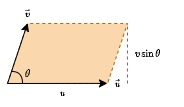
\includegraphics[]{figures/cross-product}
\end{center}

Overview
\begin{itemize}
    \item $||\textbf{a}\times \textbf{b}||=||\textbf{a}||||\textbf{b}||\sin\theta$
    \item $\textbf{a},\textbf{b}\perp \textbf{a}\times \textbf{b}$
\end{itemize}

Algebraic
\begin{itemize}
    \item $\textbf{a}\times \textbf{b}=\textbf{0}$
    \item $\textbf{a}\times \textbf{b}=-\textbf{b}\times \textbf{a}$
    \item Distributive properties hold -- preserve direction however
    \item $(\alpha \textbf{a})\times \textbf{b}=\alpha(\textbf{a}\times \textbf{b})$
\end{itemize}

\section{Graphs}

\subsection{Multivariable functions}

Function of $n$-variables is real-valued function with $f(x_1,\cdots,x_n)$ with domain $\mathcal{D}$
being a set of $n$-tuples $(x_1,\cdots,x_n)$ in $\R^n$, or where $f$ is defined.
Range of $f$ is all values $f(x_1,\cdots,x_n)$ for $(x_1,\cdots,x_n)$ in the domain.

\subsection{Graphing multivariable functions}

Traces are 2D curves obtained by intersection with planes parallel to coordinate plane.
\begin{itemize}
    \item Horizontal trace at height $c$ -- intersection of graph with plane $z=c$, so points $(x,y,c)$ such that $f(x,y)=c$
    \item Vertical trace in plane $x=a$ -- intersection of graph with vertical plane $x=a$ for all points $(a,y,f(a,y))$
    \item Vertical trace in plane $y=b$ -- intersection of graph with vertical plane $y=b$ for all points $(x,b,f(x,b))$
\end{itemize}

\begin{center}
    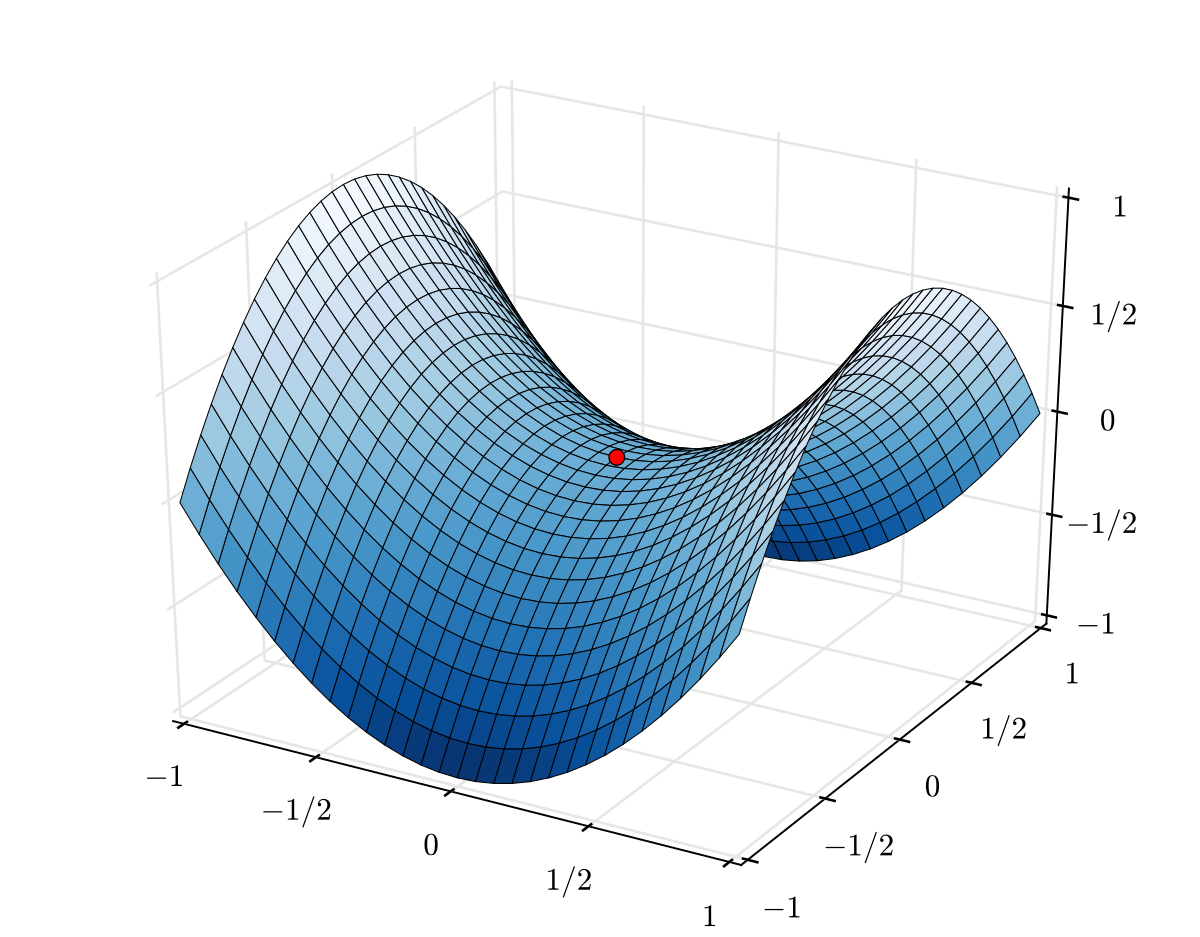
\includegraphics[scale=0.15]{figures/saddle-plot.png}
\end{center}

Saddle surface general form is $f(x,y)=x^2-y^2$. The horizontal traces are hyperbolas of the form $c=x^2-y^2$.
Vertical traces are parabolas, as either $x,y$ set to 0.\newline

\noindent
Linear functions in 2 variables are of the form $f(x,y)=mx+ny+r|m,n,r\in \R$.

\subsection{Contour maps and level curves}

\begin{center}
    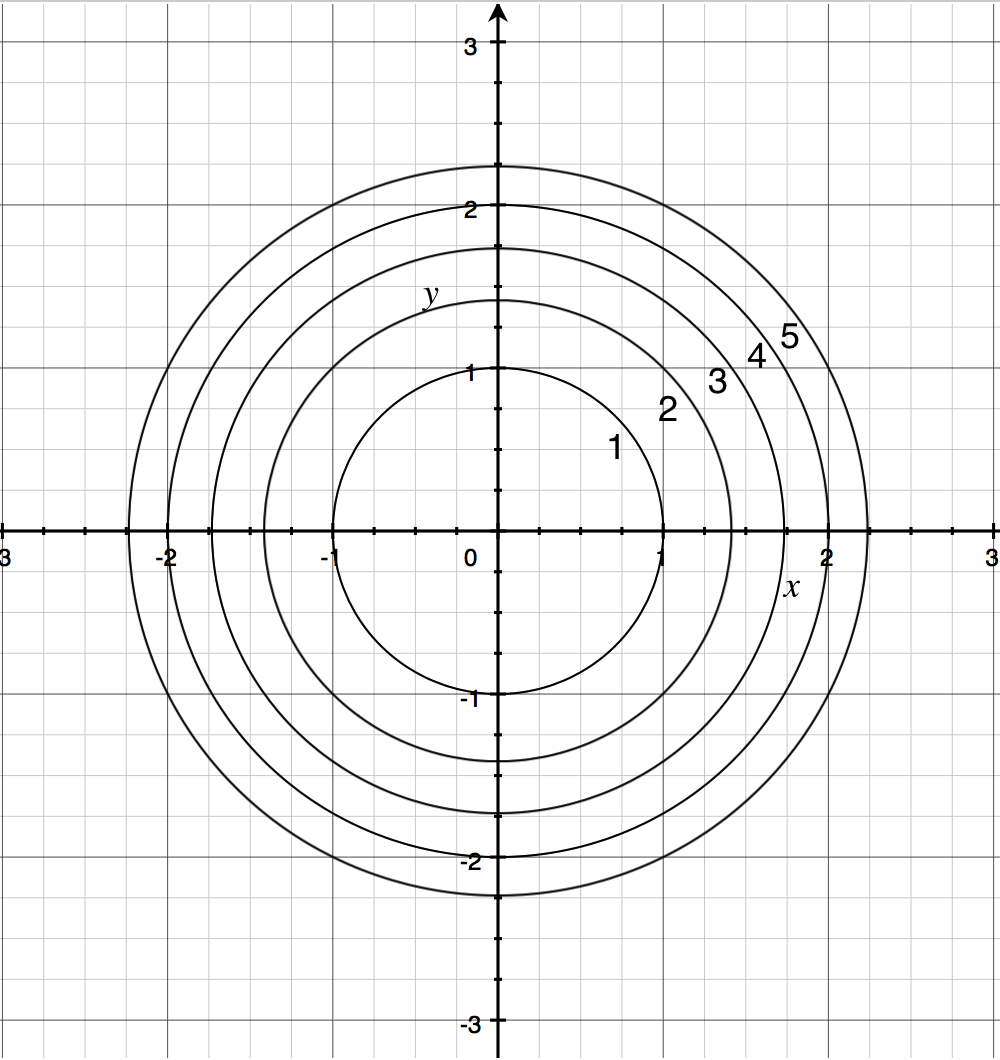
\includegraphics[scale=0.15]{figures/contour-map.png}
\end{center}

Can specify a contour interval for each $z=c$ value. Is a 2D representation of
level curves of $f(x,y)$ at an interval. Going along level curve means change in altitude is
0. Altitude has change of $\pm m$ (contour interval) when going up/down contour levels. Average ROC is $\Delta \text{elevation}/\Delta \text{distance}$.
Path of steepest ascent follows the shortest possible segment from one contour line to another and always points in steepest direction.

\begin{center}
    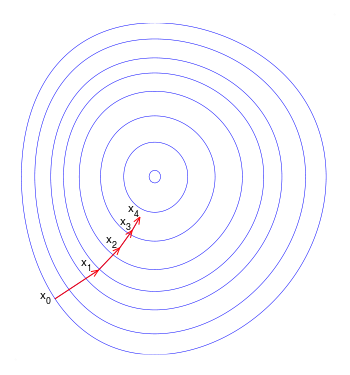
\includegraphics[scale=0.3]{figures/steepest-ascent.png}
\end{center}

\section{Partial Derivatives}

\subsection{Definition}

If $f:\R^2\rightarrow \R$ is given by $f(x,y)=z$ abd $P_0=(a,b)$ is a point in the domain of $f$,
then the partial derivative are:
\begin{itemize}
    \item If $h:\R\rightarrow \R$ by $h(t)=f(t,b)$, then partial derivative with respect to $x$ at $P_0$
    is $h\,'(a)$ with following limit definition

    \[\left.\frac{\partial f}{\partial x}\right|_{(a, b)}=f_{x}(a, b)=\lim _{h \rightarrow 0} \frac{f(x+h, b)-f(x, b)}{h}=\lim _{x \rightarrow a} \frac{f(x, b)-f(a, b)}{x-a}\]

    \item If $g:\R\rightarrow \R$ by $g(t)=g(t,b)$ then partial derivative with respect to $y$ at $P_0$ is $g\,'(b)$ with following limit definition
    
    \[\left.\frac{\partial f}{\partial y}\right|_{(a, b)}=f_{y}(a, b)=\lim _{h \rightarrow 0} \frac{f(a, x+h)-f(a, b)}{h}=\lim _{y \rightarrow b} \frac{f(a, y)-f(a, b)}{y-b}\]

\end{itemize}

Can be thought of as the intersection of the plane shifted by $b$ with $f$, and the derivative of the resulting trace.

\subsection{Linear approximation with planes}

Let $z=f(x,y)$ be a scalar-valued function in $\R^2$ and $P_0=(a,b)$ be a point in domain of $f$. Can have 2 slope vectors representing partial derivatives:
$(1,0,f_x(a,b))$ and $(0,1,f_y(a,b))$. Can find a linear approximation by finding set of points in plane spanned by these vectors passing through
$(a,b,f(a,b))$.

\[\textbf{n}=(1,0,f_x(a,b))\times(0,1,f_y(a,b))=(-f_x(a,b),-f_y(a,b),1)\]

Building the plane:

\begin{align*}
    (x-a, y-b, z-f(a, b)) \cdot \textbf{n} &=0 \\
    (x-a, y-b, z-f(a, b)) \cdot\left(-f_{x}(a, b),-f_{y}(a, b), 1\right) &=0 \\
    -f_{x}(a, b)(x-a)-f_{y}(a, b)(y-b)+z-f(a, b) &=0
\end{align*}

Thus,

\[z=f(a, b)+f_{x}(a, b)(x-a)+f_{y}(a, b)(y-b)\]

\subsection{Higher-order derivatives}

Can be calculated using derivatives of $f_x$ and $f_y$. Notation:

\[f_{xx}=\frac{\partial}{\partial x}(\frac{\partial f}{\partial x}),\; f_{yy}=\frac{\partial}{\partial y}(\frac{\partial f}{\partial y})\]

Can also have mixed partials (read as with respect to $x$ or $y$):

\[f_{xy}=\frac{\partial}{\partial y}(\frac{\partial f}{\partial x}),\; f_{yx}=\frac{\partial}{\partial x}(\frac{\partial f}{\partial y})\]

By Clairaut's Theorem, if $f_{xy}$ and $f_{yx}$ are both continuous functions on a disk $D$, then $f_{xy}(a,b)=f_{yx}(a,b)\: \forall (a,b)\in D$. Means that $f_{xyxy}=f_{xxyy}=f_{yyxx}=f_{yxyx}$.

\section{Extrema}

\subsection{Definition and proofs}

A function $f$ has:
\begin{itemize}
    \item local maximum at $P_0$ in domain if $f(P_0)>f(x,y)\;\forall\;(x,y)$ sufficiently near $P_0$
    \item local minimum at $P_0$ in domain if $f(P_0)<f(x,y)\;\forall\;(x,y)$ sufficiently near $P_0$
\end{itemize}

Sufficiently near: positive radius $R$ used to build a circle centered at $P_0$ that traps points in domain with desired property (min or max).
Global extrema redefine sufficiently near as in the domain of $f$.

Critical point is defined as either of the following:
\begin{itemize}
    \item $f_x(P_0)=f_y(P_0)=0$
    \item either $f_x(P),f_y(P)$ does not exist
\end{itemize}

Method: find critical value $y$ from $f_y$ and $x$ from $f_x$ through cross-substitution.

Proof that if $f_x(P),f_y(P)$ both exist and there is a local max at $P$, then both partials are 0:

Define $g:\;\R\rightarrow \R$ to be single variable function from holding $y=b$ in $f$. Considering points sufficiently near:

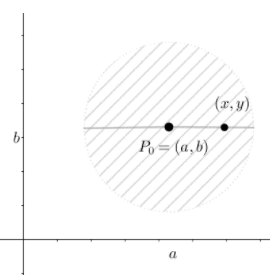
\includegraphics[scale=0.5]{figures/Screen Shot 2021-03-21 at 7.55.34 PM.png}

Plugging into function $g$: $g(x) < f(x,b) \leq f(P_0)=g(a)$, so for $x$-values sufficiently
near $a$, $g(x)\leq g(a)$, so it is a local max of $g$. Invoking theorem of extrema, either $g'(a)=0$ or DNE. As $g'(a)=f_x(P_0)$, demonstrates that
$f_x=0$ or DNE for a local max. Same can be done for $f_y$.

Can minimize a function's distance to origin through distance formula. As a square root minimizes
at its argument, can just concentrate on minimizing the argument.

Reiteration: If $f: \mathbb{R}^{2} \rightarrow \mathbb{R}$ has continuous first and second order partial derivatives then $f_{x y}(x, y)=f_{y x}(x, y)$.
Continuous 2nd order partials: $C^2$; continous $n$ order partials: $C^\infty$.

\textbf{Fermat's theorem proof (same as above):} If $f(x,y)$ has a local min/max at $P=(a,b)$, then $P=(a,b)$ is a critical point of $f(x,y)$.

Assuming $f(x,y)$ has a local min at $P$, then this means that $f(x,y) \geq (a,b)$ for $(x,y)$ in the surrounding disk $D(r,P)$.
For some $y=b$, the distance between any 2 $x$-values must be contained in the disk: $|x-a|<r$. Shows that $g(x)=f(x,b)$ has a local min
at $x=a$, so $g'(a)=0$ or DNE. Because $g'(a)=f_x(a,b)$, $f_x(a,b)$ is either 0 or DNE. As the same can be said for $f_y$, $P$ is a critical point.

\subsection{Second-derivative test}

Given a function $f:\R^2 \rightarrow \R$ that has continuous 2nd partials near a critical point $P$, define
the discriminant of $f$ at $P$ to be:

\[D(P)=f_{x x}(P) f_{y y}(P)-\left(f_{x y}(P)\right)^{2}\]

Then:
\begin{itemize}
    \item If $D>0$, $P$ is a local extreme of $f$
    \begin{itemize}
        \item $f_{xx}(P)>0$ implies a local min
        \item $f_{xx}(P)<0$ implies a local max
    \end{itemize}
    \item If $D<0$ then there is neither a min or max at $P$, but an inflection point (saddle point)
    \item If $D=0$ then there is no information about $P$
    \item If $D>0$ and $f_{xx}(a,b)>0$, then local minimum
    \item If $D>0$ and $f_{xx}(a,b)<0$, then local maximum
\end{itemize}

Observe that $D(P)=\operatorname{det}\left(\begin{array}{ll}
                f_{x x}(P) & f_{x y}(P) \\
                f_{y x}(P) & f_{y y}(P)
            \end{array}\right)$

\subsection{Global extrema}

If $f:\R^2 \rightarrow \R$ is continuous on a closed and bounded subset of $\R^2$ then it has a global max/min
on the subset (at critical point or along boundary)

A closed subset of $\R^2$ is one that contains the boundary. Boundary points have the property that
any circle centered around them with positive radius will contain points in and out of the subset.
Bounded subset is where any distance between 2 points in the set never exceeds some fixed bound $M\in \R$.

\begin{center}
    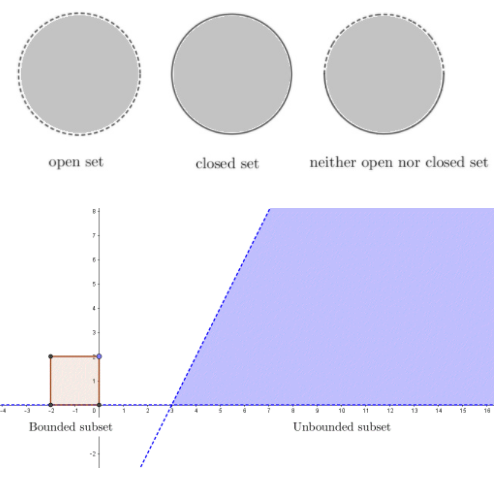
\includegraphics[scale=0.5]{figures/Screen Shot 2021-03-22 at 3.01.05 PM.png}
\end{center}

The boundary curve is denoted as $\partial D$ where $D$ is a disk. By parameterizing $\partial D$ and using function
composition to take this curve $\textbf{c}(t)$ into $f$: $h(t)=f(\textbf{c}(t))$. A min/max for $f$ along boundary curve
is a min/max of $h$. Plug resulting coordinates into $f$ and determine global extrema.

\section{Lagrange Multipliers}

\subsection{Theory}

Let $f:\R^2\rightarrow \R$ and $\textbf{c}:\R\rightarrow \R^2$ such that there is a composite function $h(t)=f(\textbf{c}(t))$.
Then, $h\,'(t)=f_x(\textbf{c}(t))x\,'(t)+f_y(\textbf{c}(t))y\,'(t)=\left(f_{x}\left(\textbf{c}(t)), f_{y} \textbf{c}(t)\right) \cdot \textbf{c}^{\prime}(t)\right.$.
This brings definition of gradient vector, so that for $f:\R^2\rightarrow \R$, each point in domain is in domain of $f$ the vector $\left(f_{x}\left(P_{0}\right), f_{y}\left(P_{0}\right)\right)$:

\[\nabla f\left(P_{0}\right)=\left(f_{x}\left(P_{0}\right), f_{y}\left(P_{0}\right)\right)\]

Rewriting chain rule:

\[\frac{d}{dt}f(\textbf{c}(t_0))=\nabla f(\textbf{c}(t_0))\cdot \textbf{c}\,'(t_0)\]

Let $g(x,y)$ be boundary curve function and $f(x,y)$ be original.

Use a boundary curve which is level curve $c=0$ which represents the boundary of the subset where global extrema can be found. 
If $f$ achieves maximum at point $P$ along curve, then either $g_x(P)=g_y(P)=0$ ($\nabla g(P)=\textbf{0}$) or there is a scalar $\lambda$ (Lagrange multiplier)
such that $f_x(P)=\lambda g_x(P)$ and $f_y(P)=\lambda g_y(P)$ ($\nabla f(P)=\lambda \nabla g(P)$). Can find locations of global extreme without parameterizing.

\subsection{Proof}

Suppose $f(P)\geq f(x,y)\;\forall\;(x,y)$ satisfying $g(x,y)=0$ where $g$ is the bounded constraint. Let $\textbf{c}$ be its parameterization where $\textbf{c}\,'(0)\neq 0$. Parameterizing $g(x,y)=0$ with $\textbf{c}(t)$
such that $\textbf{c}(0)=P$: Observe that $h(t)=f(\textbf{c}(t))$ is from $\R\rightarrow\R$ with local max at $t=0$.
Thus, $h'(t)=0$ or DNE. Taking derivative, $h'(t)=\nabla f(\textbf{c}(t))\cdot \textbf{c}\,'(t)$.
Then, $h^{\prime}(0)=\nabla f(\textbf{c}(0)) \cdot \textbf{c}^{\prime}(0)=0$ or DNE. This dot product is either 0 or DNE because
1 or both vectors could not exist, or if they are $\perp$. Thus, $\nabla f(P)\perp \textbf{c}\,'(0)$ and $\textbf{c}\,'(0)\neq \textbf{0}$ (because $\textbf{c}$ is assumed to be regular).

Showing $\nabla g(P)\perp \textbf{c}\,'(0)$. Define $j(t)=g(\textbf{c}(t))$. Thus, $j^{\prime}(t)=\nabla g(\textbf{c}(t)) \cdot \textbf{c}^{\prime}(t)$.
Because $\textbf{c}(t)$ is a parameterization of level curve $g(x,y)=0$, it always outputs 0, so $j(t)=g(\textbf{c}(t))=0$ always. Can the conclude that
$j^{\prime}(t)=\nabla g(\textbf{c}(t)) \cdot \textbf{c}^{\prime}(t)=0$. Plugging in $t=0$ gives $\nabla g(\textbf{c}(0)) \cdot \textbf{c}^{\prime}(0)=0$ so $\nabla g(P)\perp \textbf{c}\,'(0)$.

Because both vectors are perpendicular to $\textbf{c}\,'(0)$, they are parallel -- $\nabla f(P)=\lambda \nabla g(P)$. Or:

$$\begin{array}{l}
    f_{x}(P)=\lambda g_{x}(P) \\
    f_{y}(P)=\lambda g_{y}(P)
\end{array}$$
\section{Limits}

\subsection{Delta-Epsilon Definition on R}

The limit of $f$ as $x$ approaches $a$ is $L$ if given a positive real number
$\epsilon$, there exists a corresponding $\delta$ so that numbers selected with distance from $a$
less than $\delta$ and $>0$ it is guaranteed that outputs under $f$ are within distance $\epsilon$ from $L$.

Formal definition:

$\lim_{x\to a}f(x)=L$ if $\forall \epsilon >0$, $\exists\delta > 0$ such that $0< |x-a| < \delta \implies |f(x)-L|<\epsilon$

\subsection{Definition of Limit on R2}

If $f:\R^2\to \R$ and $P_0=(x_0,y_0)$, then $\lim _{(x, y) \rightarrow\left(x_{0}, y_{0}\right)} f(x, y)=L$ 
if given any small positive number $\epsilon$, $\delta>0$ is guaranteed so when there is a point $C\neq P_0$ within circle of radius $\delta$ about $P_0$, $f(x,y)$ lies within $\epsilon$ of $L$.

Formally: 

\[\lim _{(x, y) \rightarrow\left(x_{0}, y_{0}\right)} f(x, y)=\lim _{\tb{x} \rightarrow P_{0}} f(x, y)=L \text { if } \forall \varepsilon>0 \;\exists \delta>0\]

such that

\[0<\sqrt{\left(x-x_{0}\right)^{2}+\left(y-y_{0}\right)^{2}}<\delta \Longrightarrow|f(x, y)-L|<\varepsilon\]

\subsection{Continuous Functions}

\begin{itemize}
    \item Polynomials: $f(x,y)=x^2y+xy^2$
    \item Exponentials: $f(x,y)=e^{xy}$
    \item Trigonometric: $f(x,y)=\sin(x+y)$
    \item Compositions of any continuous functions: $f(x,y)=\cos(e^{x^2y-xy^2})$
    \item Sums, differences, products of continuous functions: $f(x, y)=x^{2} y-x y^{2}+e^{x y} \sin (x y)$
    \item Quotients of continuous functions (domain of quotient does not include zeros of denominator): $f(x, y)=\frac{x^{2 y}-x y^{2}}{\sin (x y)}$
\end{itemize}

\subsection{Computational Techniques}

Can use continuity to find limit (plug in point). Can also use conjugate multiplication to simplify and compute. Cancelling terms works because a limit approaches a value instead of equaling it.
Can also squeeze a function between 2 continuous ones to find limit.

Let $\lim _{(x, y) \rightarrow(0,0)} \frac{x^{2}}{\sqrt{x^{2}+y^{2}}}$ exist.
Know that $0\leq \lim _{(x, y) \rightarrow(0,0)} \frac{x^{2}}{\sqrt{x^{2}+y^{2}}}$.
Because $y^2>0$, $\frac{x^{2}}{\sqrt{x^{2}+y^{2}}} \leq \frac{x^{2}+y^{2}}{\sqrt{x^{2}+y^{2}}}$.
Thus, $\lim _{(x, y) \rightarrow(0,0)} 0 \leq \lim _{(x, y) \rightarrow(0,0)} \frac{x^{2}}{\sqrt{x^{2}+y^{2}}} \leq \lim _{(x, y) \rightarrow(0,0)}\left(x^{2}+y^{2}\right)^{1 / 2}$
so the limit is 0.

Other strategies: If a term $k(x,y)\geq 0\;\forall\; (x,y)\in \R^2$, then can simply perform $\pm 1$ to denominator for squeeze theorem proofs.

\subsection{Common inequalities and proofs}

\begin{itemize}
    \item AM-GM inequality: $\frac{x+y}{2}\geq \sqrt{xy}\implies (x-y)^2\geq 0$
    \item Triangle inequality: $|x+y|\leq |x|+|y|$ and $|x-y|\geq |x|-|y|$
    \item $|e^x-1|\leq |x|e^{|x|}$
\end{itemize}

Proof that $\frac{\sin x}{x}=1$:

\begin{center}
    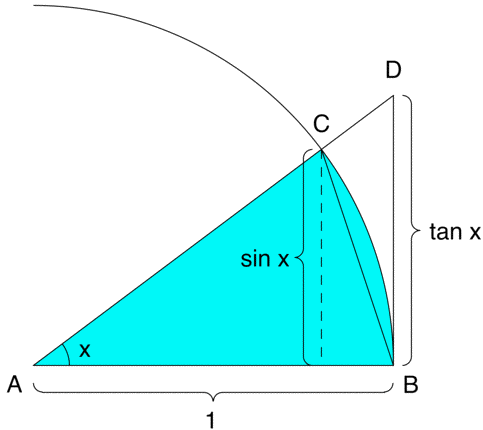
\includegraphics[scale=0.4]{Screen Shot 2021-04-21 at 10.59.12 AM.png}
\end{center}

It is evident that:
\begin{gather}
    \frac{1}{2}\sin x\leq \frac{1}{2}x\leq \frac{1}{2}\tan x\\
    \sin x\leq x \leq \tan x\\
    1\leq \frac{x}{\sin x}\leq \frac{1}{\cos x}\\
    1\geq \frac{\sin x}{x}\geq \cos x
\end{gather}

Applying the squeeze theorem to 4:

\begin{gather*}
    \lim_{x\to 0}1\geq \lim_{x\to 0}\frac{\sin x}{x}\geq \lim_{x\to 0} \cos x\\
    1\geq \frac{\sin x}{x}\geq 1
\end{gather*}

Thus, $\lim_{x\to 0}\frac{\sin x}{x}=1$.

\section{Derivatives}

\subsection{Limit Definition}

A function $f:\R^m \to \R^n$ is differentiable at $P_0$ if there is a linear transformation from $n\times m$ matrix $Df(P_0)$ satisfying

\[\lim_{\tb{x}\to P_0}\frac{\big\vert \big\vert f \big( \tb{x} \big)-\big(f(P_0)+\mathrm{D}f(P_0)(\tb{x}-P_0) \big) \big\vert \big\vert}{\vert \vert \tb{x}-P_0 \vert \vert}=0\]

If the function is differentiable at this point, then $Df(P_0)$ is the derivative of $f$ at $P_0$. Called Jacobian matrix of $f$ at $P_0$.

Can adapt this to single-variable calculus:

\[\displaystyle \lim_{x\to a} \frac{\vert f(x)-\big(f(a)+(m_a)(x-a)\big) \vert}{\vert x-a \vert}=0\]

Simplifying and reconfiguring to limit definition of a derivative:

\begin{align*}
    \lim_{x\to a} \frac{\vert f(x)-\big(f(a)+(m_a)(x-a)\big) \vert}{\vert x-a \vert}&=0\\
    \lim_{x\to a}\left\vert \frac{f(x)-\big(f(a)+(m_a)(x-a)\big)}{x-a} \right\vert&=0\\
    \left \vert \lim_{x\to a} \frac{f(x)-\big(f(a)+(m_a)(x-a)\big)}{x-a} \right \vert&=0\\
    \lim_{x\to a} \frac{f(x)-\big(f(a)+(m_a)(x-a)\big)}{x-a}&=0 \, \mbox{since}\, \vert 0 \vert=0\\ 
    \lim_{x\to a} \left( \frac{f(x)-f(a)}{x-a}-m_a\right)&=0\\
    \lim_{x\to a}\frac{f(x)-f(a)}{x-a}&=m_a
\end{align*}

Equivalent to the case of a $1\times 1$ matrix $Df(P_0)$ where the single entry is $f'(a)$.
Also $m_a=f'(a)\implies f(x)=f(a)+f'(a)(x-a)$ is the linear approximation. 

As $x$-values approach $a$, $f(x)-(f(a)+f'(a)(x-a))$ approaches 0 faster. Thus, $\frac{f(x)-\big(f(a)+f'(a)(x-a)\big)}{x-a}$ approaches 0.

\subsection{Multivariable Application}

Approximating plane of some $f:\R^2\to \R$ is $L_{P_0}(x,y)=f(a,b)+f_x(a,b)(x-a)+f_y(a,b)(y-b)$, i.e. the plane spanned by
$\langle 1,0,f_x(a,b)\rangle$ and $\langle 0,1,f_y(a,b)\rangle$ passing through $(a,b,f(a,b))$.

Is identical to $\begin{bmatrix}f_x(P_0)&f_y(P_0)\end{bmatrix}\begin{bmatrix}x-a\\y-b\end{bmatrix}$. The matrix is the matrix of partial derivatives.

Such a function is differentiable if:

\[\displaystyle \lim_{(x,y)\to(a,b)}\frac{f(x,y)-\left(f(a,b)+\Big(\begin{matrix} f_x(a,b)&f_y(a,b) \end{matrix} \Big)\left(\begin{matrix}x-a\\y-b\\ \end{matrix} \right) \right)}{\sqrt{(x-a)^2+(y-b)^2}}=0\]

Numerator is linear approximation and denominator is distance to point $(a,b)$. Thus:

\[\boxed{f(x,y) \mbox{ is differentiable at the point }P_0\mbox{ if}\displaystyle \lim_{(x,y)\to P_0}\frac{|f(x,y)-L_{P_0}(x,y)|}{||(x,y)-P_0||}=0}\]

Geometrically, if a circle about $P_0$ is drawn and radius is collapsed, distance between $f$ and approximating plane will become 0 much faster, so fraction becomes 0.

If there is a radius $\delta > 0$ on the disk of radius $\delta$ centered at $P_0$, $f_x(x,y)$ and $f_y(x,y)$ are continuous at every point on the disk, then $f(x,y)$ is continuous at every point on the disk.
Differentiability can not be established by the existence of partial derivatives at a point, it is sufficient to demonstrate continuous partials
at a point.

The criteria for differentiability are that $f_x,f_y$ exist and $f$ is locally linear at $P_0$. The tangent plane exists here. However,
it is sufficient to demonstrate differentiability by showing that both $f_x$ and $f_y$ are continuous on an open disk $D$ to conclude that $f(x,y)$
is differentiable on $D$. Alternatively, the above limit definition can be used.

If a function $f:\R^m\to \R^n$ exists, then it is made up of $n$ component functions on $\R^m$. The Jacobian matrix is as follows:

\[Df\left( x_1,\ldots x_m\right) =\begin{bmatrix} \nabla f_{1}\left(x_1,\ldots x_m\right) \\ \vdots \\ \nabla f_{n}\left(x_1,\ldots x_m\right) \end{bmatrix}\]

The number of rows $n$ depends on components (codomain) of the output space whereas the domain determines columns ($m$). Thus, linear approximation to a function $f:\R^m\to \R^n$ at $P_0$ is

\[L_{P_0}(\tb{x})=f(P_0)+\Big(\mbox{matrix of partial derivatives at}\,P_0\Big)(\tb{x}-P_0)\]

In parametric equations (paths), let $\tb{c}(t)=\big(x(t), y(t), z(t) \big)$ have continuous partials.
Thus, the matrix of partials $D\tb c(t)=\begin{bmatrix}x'(t)\\y'(t)\\z'(t)\end{bmatrix}$. Is the vertical velocity vector.
If the approximation $L_{t_0}(t)$ is found, it yields:

\begin{align*}
    L_{t_0}(t)&=\tb c(t_0)+
    \left(
    \begin{matrix}
    x'(t_0)\\
    y'(t_0)\\
    z'(t_0)\\
    \end{matrix}
    \right)
    (t-t_0)\\
    &=\tb{c} (t_0)+(t-t_0)\tb c\,'(t_0)
\end{align*}

Also, note that matrix of partials for a scalar valued function $f:\R^n\to \R$ is simply the gradient; there is 1 row and $n$ columns in the gradient vector.

\section{Derivative Rules}

\subsection{Fundamental Rules}

If $f,g:\R^m\to \R^n$ are differentiable at $P_0\in \R^m$ for $c\in \R$:
\begin{itemize}
    \item $h(\tb{x})=cf(\tb{x})\implies \mathrm{D}h(P_0)=cDf(P_0)$
    \item $h(\tb{x})=f(\tb{x})+g(\tb{x})\implies \mathrm{D}h(P_0)=\mathrm{D}f(P_0)+\mathrm{D}g(P_0)$ (domain = codomain; sum of two $n\times m$ matrices)
\end{itemize}

If $f,g:\R^n\to \R$ are differentiable at $P_0\in \R^n$:
\begin{itemize}
    \item $h(\tb{x})=f(\tb{x})g(\tb{x})\implies \mathrm{D}h(P_0)=f(P_0)\mathrm{D}g(P_0)+g(P_0)\mathrm{D}f(P_0)$ (no commutativity as matrix times scalar DNE)
\end{itemize}

If $f,g:\R^n\to \R$ are both differentiable at $P_0\in \R^n$ and $g(P_0)\neq 0$:
\begin{itemize}
    \item $\mathrm{D}\left(\frac{f}{g}\right)(P_0)=\frac{g(P_0)\mathrm{D}f(P_0)-f(P_0)\mathrm{D}g(P_0)}{g(P_0)^2}$
\end{itemize}

\subsection{Chain Rule}

If $g:\R^m\to \R^p$ and $f:\R^p\to \R^n$ and $g$ is differentiable at $P_0\in \R^m$ and the same for $f$ at $g(P_0)$:
\begin{itemize}
    \item $\mathrm{D}\Big(f\circ g\Big)(P_0)=\mathrm{D}f\big(g(P_0)\big)\mathrm{D}g(P_0)$
\end{itemize}

Thus, derivative of composites is a matrix product. $\mathrm{D}f(g(P_0))\to n\times p$ and $\mathrm{D}g(P_0)\to p\times m$
so $\mathrm{D}(f\circ g)(P_0)\to n\times m$.

If $\tb{c}:\R\to \R^n$ is a path differentiable at $t_0\in \R$ and $f:\R^n\to \R$ is differentiable at $\tb{c}(t_0)$, then:

\[\frac{d}{dt}f(\tb{c}(t_0))=\mathrm{D}f(\tb{c}(t_0))D\tb{c}(t_0)=\left[ \nabla f\left( x_{1},x_{2},\ldots x_{n}\right) \right]\begin{bmatrix} \vdots \\ \tb{c}\,'(t_0) \\ \vdots \end{bmatrix}=\nabla f(\tb{c}\,'(t_0))\cdot \tb{c}\,'(t_0)\]

Thus, derivative of scalar valued function and path is dot product of gradient and velocity.

\section{Gradient}

\subsection{Directional Derivative}

Directional derivative of a scalar function $f:\R^n\to \R$ at some $P_0\in\R^n$ in the direction of $\tb{v}\in\R^n$ is given by

\[\boxed{f_{\tb{v}}\left(P_{0}\right)=\nabla f\left(P_{0}\right) \cdot \frac{\tb{v}}{\|\tb{v}\|}}\]

Maximizing the directional derivative involves the dot product. Let $f:\R^n\to \R$ and $P_0\in\R^n$ where $\nabla f(P_0)$ is defined.
Also, let $\tb{u}$ be a unit vector such that $f_{\tb{u}}(P_0)$ is maximized. The directional derivative is

\[f_{\tb u}(P_0)=\nabla f(P_0)\cdot \tb u=\|\nabla f(P_0)\|\cos \theta\]

Since $\cos\theta \in [-1,1]$, the directional derivative is maximized at $\cos\theta = 1\implies \tb{u}||\nabla f(P_0)$.
\textbf{Thus the gradient of a function at $P_0$ points in the direction of steepest ascent}.

For a more general case given $f:\R^n\to \R$ and $P_0\in\R^n$ where $\nabla f_{\tb{v}}(P_0)$ is maximized and $\nabla f(P_0)$ exists:
\begin{align*}
    \nabla f_{\tb{v}}(P_0)&=\nabla f(P_0) \cdot \frac{\tb{v}}{||\tb{v}||}\\
    &=\nabla f(P_0) \cdot \frac{\nabla f(P_0)}{||\nabla f(P_0)||}\\
    &=\frac{\nabla f(P_0)\cdot \nabla f(P_0)}{||\nabla f(P_0)||}\\
    &=||\nabla f(P_0)||
\end{align*}

Thus, the length of the gradient vector tells how steep the ascent is in the direction of the steepest ascent.

\subsection{Gradient Fields}

A image in the codomain $\R^n$ where arrows originating at each point point in the steepest direction $\forall\; P\in \R^n$ where the partials exist.
Are always perpendicular to level curves of $f$.

Let $f:\R^n\to \R$ and $P\in \R^n$ a point where partials of $f$ exist. Considering the level set $f(\tb{x})=f(P)$,
all values map to same codomain value as $P$. Also, let $\tb{c}:\R^n\to \R$ have an image entirely within this level set $f(\tb{x})=f(P)$
and $\tb{c}(t_0)=P$. Then, the proof must show that $\nabla f(P)\cdot \tb c\,'(t_0)=0$.

Note that since $h(t)=f(\tb{c}(t))$, $h'(t_0)=\nabla f \Big(\tb c (t_0) \Big)\cdot \tb c\,'(t_0)=\nabla f (P)\cdot  \tb c\,'(t_0)$.
Since the image of $\tb{c}(t)$ lies within $f(\tb{x})=f(P)$, $f$ is constant on the image of $\tb{c}$ (every point on $\tb{c}$ maps to $f(P)$ under $f$).
Thus, $h(t)=f(\tb{c}(t))\implies h'(t)=0\;\forall\;t$.

\subsection{Sphere}

Sphere is not a function as a point $P=(x,y)$ correspond to multiple $z$ values.
Can be viewed as a level surface in $\R^3$ for some $f:\R^3\to \R$. The function is $f(x,y,z)=x^2+y^2+z^2$
and the level surface sphere is $x^2+y^2+z^2=R^2$ where $R$ is the radius.
Given the point $(0,0,R)$, the gradient is upward along the $z$-axis. All curves passing through this point
have a tangent vector perpendicular to $\nabla f(0,0,R)$ since gradients are perpendicular to level sets.
It can be sadi that any vector perpendicular to $\nabla f(0,0,R)$ is a tangent to at least 1 curve in the sphere passing through $(0,0,R)$.
Thus, the perpendicular space to $\nabla f(0,0,R)$ forms a plane of tangent vectors at $(0,0,R)$ and is a tangent plane.
An expression for the tangent plane is 

\begin{align*}
    \nabla f (0,0,R)\cdot(x-0, y-0, z-R)&=0\\
    f_x(0,0,R)x+f_y(0,0,R)y+f_z(0,0,R)&=0\\
    2(0)x+2(0)y+2(R)(z-R)&=0\\
    2Rz-2R^2&=0\\
    z&=R\\
\end{align*}

Expression for the tangent plane to a level set of some $f:\R^3\to \R$:

\begin{align*}
    \nabla f (P_0)\cdot(x-x_0, y-y_0,z- z_0)&=0\\
    f_x(P_0)(x-x_0)+f_y(P_0)(y-y_0)+f_z(P_0)(z-z_0)&=0\\
    f_x(P_0)x+f_y(P_0)y+f_z(P_0)z&=\nabla f(P_0)\cdot P_0\\
\end{align*}
$$\boxed{f_x(P_0)x+f_y(P_0)y+f_z(P_0)z=\nabla f(P_0)\cdot P_0}$$

% -------------------------------------
\end{document}